\documentclass[main.tex]{subfiles}
\begin{document}

\begin{center}
\Large Criptografía y Seguridad (72.44)\\[.05cm]
Bell-La Padula: Modelo de Confidencialidad \\[.05cm]
\the\year
\end{center}

\vspace{0.2 cm}
\iffalse
\section{Control de Accesos}
Normalmente en sistemas operativos primero se autentica a los principales
(mediante algún mecanismo como contraseñas, o Kerberos), y posteriormente se
media el acceso de estos a recursos, como pueden ser archivos, puertos, etc.
Estos controles de acceso pueden modelarse con una matriz de permisos de acceso,
donde las columnas se usan para archivos, y las filas para los usuarios.

Estas matrices de control de accesos se pueden utilizar tanto para modelar, como
para implementar mecanismos de protección, pero tienen la desventaja de no ser
escalables (por ejemplo, una multinacional con 40.000 empleados y unos 1.000 recursos
a los que mediar su acceso, requeriría una matriz de 40.000.000 de entradas). 

En general, es preferible usar métodos más compactos de almacenar y administrar
esta información, y para esto se suele comprimir los usuarios, o comprimir los
permisos.

Para comprimir usuarios, se suele utilizar grupos o roles para administrar los
privilegios de un conjunto de usuarios.

Para comprimir los permisos, existen dos formas de almacenar la matriz
de control de accesos:
\begin{enumerate}
  \item Por columnas, junto con el recurso al que la columna hace referencia.
    Esto se conoce como listas de control de accesos (ACL, pronunciadas
    ``ackle'' en inglés).
  \item Por filas, conocidas como capacidades (\textit{capabilities}, o en menor
    medida \textit{tickets}).
\end{enumerate}

\begin{table}[h!]
  \centering
\begin{tabular}{l|c|c|c} 
 Usuario & apuntes.tex & apuntes.pdf & script.sh \\ 
 \hline
 Alice   & \verb+rw+   & \verb+r+    & \verb+-+ \\ 
 Bob     & \verb+r+    & \verb+r+    & \verb+rx+ \\ 
 Charlie & \verb+-+    & \verb+-+    & \verb+rwx+ \\
\end{tabular}
\caption{Lista de control de accesos (ACL).}
\end{table}

En Unix (y Linux), los archivos no


Acceso Discrecional
Acceso Mandatorio

En Unix, write access no implica read access. Aplicados a un directorio,
significan:
- read: listar el contenido del directorio;
- write: crear o renombrar un archivo en el directorio;
- execute: buscar el directorio;

formal statement of your security policy = A security model.

Los PKI son una reimplementación de un viejo concepto de control de accesos:
capacidades.

\fi

%\section{Bell-La Padula: Modelo de Confidencialidad}

Durante los comienzos de los 70, la Fuerza Aérea de Estados Unidos tenía sus
preocupaciones con respecto a la seguridad de los sistemas de computadoras
centrales de tiempo compartido (\textit{time-sharing mainframe systems}). 
En respuesta a esto,  Bell y La Padula propusieron en una serie de reportes un
modelo de política de seguridad \cite{BLP73, BLP73b, Bell74}. Lo desarrollado en estos fue
posteriormente resumido y adaptado a Multics en un reporte final \cite{BLP76}.
El modelo Bell-La Padula (BLP) es una política de seguridad multinivel
(\textit{multilevel security policy}) basado en máquinas de estado.  Define
formalmente qué significa que un estado sea ``seguro'', y analiza qué
transiciones de estado son permisibles de forma que un estado seguro no lleve a
uno inseguro. 

El objetivo de BLP es prevenir la divulgación indebida de información; en una
palabra, confidencialidad. El problema esencial que busca resolver es controlar
el acceso de entidades activas llamadas sujetos, a un conjunto de entidades
pasivas (protegidas) llamadas objetos. Más formalmente, el modelo consta de:
\begin{itemize}
\itemsep0em 
  \item Un conjunto de sujetos $S$ (\textit{subjects}).
  \item Un conjunto de objetos $O$ (\textit{objects}).
  \item Una matriz de accesos (\textit{access matrix}), donde la celda $a_{ij}$
    contiene los permisos de acceso del sujeto $s_i$ sobre el objeto $o_j$.
    \begin{table}[h!]
      \centering
    \begin{tabular}{c|ccc} 
      & $o_1$ & $\cdots$ & $o_m$ \\ 
     \hline
     $s_1$   & \texttt{\underline{r}}   &    & \verb+-+ \\ 
     $\vdots$     &   & $\ddots$  &  \\ 
     $s_n$ & \texttt{\underline{rw}} &    & \texttt{\underline{e}} \\
    \end{tabular}
    \end{table}
    
    A
    los distintos permisos se los conoce como atributos o modos de acceso, y
    pueden ser \texttt{\underline{e}}, \texttt{\underline{r}},
    \texttt{\underline{a}}, o \texttt{\underline{w}}.
  \item Un conjunto de clasificaciones de seguridad, con un orden parcial
    $\leq$. Las clasificaciones son, en orden creciente: \textit{Unclassified}
    (U), \textit{Confidential} (C), \textit{Secret} (S) y \textit{Top Secret} (TS).
  \item Un conjunto de categorías (\textit{categories}).
\end{itemize}

Los sujetos suelen ser usuarios, o más generalmente procesos. Los objetos son
habitualmente archivos, dispositivos y otras entidades implementadas por un
sistema operativo.
El conjunto de atributos de acceso surge de que hay dos efectos que un acceso
puede tener sobre un objeto:
\begin{enumerate}
\itemsep0em 
  \item Extraer información (``observar'' el objeto).
  \item Introducir información (``alterar'' el objeto).
\end{enumerate}
Por lo tanto, hay cuatro tipos generales de acceso imaginables:
\begin{enumerate}
\itemsep0em 
  \item Ni observar, ni alterar; acceso \texttt{\underline{e}}.
  \item Observar sin alterar; acceso \texttt{\underline{r}}.
  \item Alterar sin observar; acceso \texttt{\underline{a}}.
  \item Observar y alterar; acceso \texttt{\underline{w}}.
\end{enumerate}
Como es deducible, las letras usadas para los atributos de acceso derivan de
\verb+execute+, \verb+read+, \verb+append+ y \verb+write+, pero su significado
no necesariamente concuerda con el mencionado anteriormente. Por ejemplo,
ejecutar un programa requiere que la computadora lea (observe) las instrucciones
del mismo, y de hecho en Multics el atributo \texttt{\underline{e}} requiere
tanto permisos de ejecución como lectura. Distintas implementaciones modifican o
agregan permisos, pero estos cuatro son los básicos.

La clasificación (a veces llamado \textit{sensitivity level}), busca
separar la información de acuerdo a qué tan sensible es (en un ámbito militar,
en base al costo posible de que la información se filtre a un enemigo). Si bien
los cuatro niveles listados son los originales del modelo, se puede usar
cualquier cantidad de niveles. Por su parte, las categorías surgen del principio \textit{need-to-know}. La idea es que
no debería encomendarsele información clasificada a alguien salvo que
además de tener la autorización suficiente, tenga alguna necesidad particular de conocerla relacionada
a su trabajo. Por ejemplo, el teniente general del Ejercito Argentino, y el
almirante de la Armada Argentina pueden ambos tener la misma autorización de
seguridad (e.g. \textit{Top Secret}), pero uno no tiene (en general) porqué tener acceso a la
información del otro. Para contemplar esto se agregan las etiquetas
denominadas categorías. A cada sujeto y objeto se le asigna un nivel de
seguridad (\textit{security level}), que es un par (Clasificación, Categorías).
Para que un sujeto pueda observar un objeto, es necesario que su nivel de
seguridad domine al nivel de seguridad del objeto. La relación de
dominancia $\mathsf{dom}\colon L\times L \to \{0,1\}$ es un orden parcial, y se define como:
\[ (c_1,~K_1)~\mathsf{dom}~(c_2,~K_2) \Longleftrightarrow c_1 \geq c_2~\wedge~K_1 \supseteq K_2\] 
donde $c_1, c_2$ son clasificaciones, y $K_1, K_2$ son conjuntos de categorías.
El conjunto partes $\mathcal{P}(K)$ de las categorías junto con la
relación $\subseteq$ forman un retículo. Por ejemplo, dado el conjunto
$K=~$\mbox{\{A, B, C\}} de categorías, se tiene el retículo de la \autoref{fig:hasse},
donde $\emptyset \subseteq$ \{A\}, \{A\} $\subseteq$ \{A,B\}, pero \{A\}
$\nsubseteq$ \{B\}, etc.; el supremo es \mbox{\{A, B, C\}}, y el ínfimo es
$\emptyset$. También forman un retículo los niveles de seguridad (pares clasificación-categorías) con la relación de dominancia $\mathsf{dom}$.

\begin{figure}[htp]
  \centering
\begin{minipage}{.46\textwidth}
  \centering
  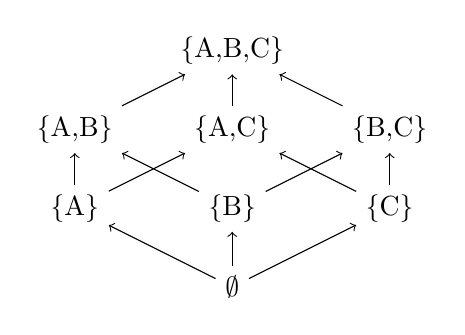
\begin{tikzpicture}
    \node at (2,3) (ABC) {\{A,B,C\}};
    \node at (4,2) (BC) {\{B,C\}};
    \node at (2,2) (AC) {\{A,C\}};
    \node at (0,2) (AB) {\{A,B\}};
    \node at (4,1) (C) {\{C\}};
    \node at (2,1) (B) {\{B\}};
    \node at (0,1) (A) {\{A\}};
    \node at (2,0) (E) {$\emptyset$};
    \draw[<-] (ABC) -- (AB);
    \draw[<-] (ABC) -- (AC);
    \draw[<-] (ABC) -- (BC);
    \draw[<-] (AC) -- (C);
    \draw[<-] (BC) -- (C);
    \draw[<-] (AB) -- (B);
    \draw[<-] (BC) -- (B);
    \draw[<-] (AB) -- (A);
    \draw[<-] (AC) -- (A);
    \draw[<-] (C) -- (E);
    \draw[<-] (B) -- (E);
    \draw[<-] (A) -- (E);
  \end{tikzpicture}
  \caption{\label{fig:hasse} Diagrama de Hasse del retículo formado por $\mathcal{P}(K)$ y la
  relación de orden $\subseteq$, representada mediante flechas.}
\end{minipage}
\end{figure}

%Se dice que un objeto tiene una clasificación de seguridad (\textit{security
%classification}), mientras que un sujeto cuenta con una autorización de seguridad (\textit{security clearance}), que determina a qué documentos tiene acceso.
Haciendo abuso de notación\footnote{Ya que los dominios son distintos.
  Formalmente, se hace uso de dos funciones $f_O\colon O \to L$ y $f_S\colon S
\to L$, donde $L$ es el conjunto de niveles de seguridad.} por simplicidad,
denotamos con $L(s)$ el nivel de seguridad de un sujeto $s$, y con $L(o)$ el 
nivel de seguridad de un objeto $o$. Acordado esto, se definen dos
características del sistema, y se refiere colectivamente a estas como
``seguridad''. La primera de estas es:
\begin{enumerate}
  \item \textbf{Propiedad simple de seguridad\footnotemark:} $s$ puede leer $o$ sii $L(s)~\mathsf{dom}~L(o)$ y $s$ tiene permisos para leer $o$. 

\footnotetext{\textit{Simple security property (ss-property)}, también conocida como \textit{no-read-up policy} (NRU).} 

    Es decir, ningún proceso puede leer datos en un nivel mayor. En la primera
    versión del modelo (\cite{BLP73}), seguridad se refería solo a esta
    propiedad.  Pero, ¿qué pasa si por ejemplo un usuario se encuentra infectado
    con un troyano, y accede a un documento? Este programa podría escribir en un
    documento a un nivel de seguridad menor que el documento original,
    efectivamente filtrando información como se observa en la
    \autoref{fig:star}. Por esto, se agregó luego la propiedad siguiente.
  \item \textbf{Propiedad-* (estrella)\footnotemark:} $s$ puede escribir $o$ sii $L(o)~\mathsf{dom}~L(s)$ y $s$ tiene permisos para escribir $o$.

Es decir, ningún proceso puede escribir datos en un nivel menor.\footnotetext{\textit{Star property (*-property)}, también conocida como \textit{no-write-down policy} (NWD). Sobre el origen del nombre, Bell dijo: \textit{I scribbled the heading ``*-property'' on the blackboard [..] After a burst of energetic discussion, I pointed out that if we didn't change the name right then, we'd be stuck with it forever. Nothing came to us and we continued our discussion. ``*-property'' it remained.} \cite{B12} } 
\end{enumerate}


\begin{figure}[htp]
  \centering
  \begin{minipage}{.7\textwidth}
  \begin{tikzpicture}
    \node [ellipse,draw, minimum width=2cm, minimum height=1cm] (o1) at (9,3) {Objeto 1};
    \node [ellipse,draw, minimum width=2cm, minimum height=1cm] (o2) at (9,0) {Objeto 2};
    \node (c) at (1,2.5) {\textit{Confidential} };
    \node (u) at (1,.5) {\textit{Unclassified} };
    \node [rectangle, draw] (s) at (4,3) {Sujeto malicioso};
    \node [color=darkblue, text width=3cm] (f) at (8.7,2.2) {%
      \hyphenchar\font=-1 % turn of hyphenation globally
    Flujo de información};
    \draw[<-] (o1) to node[above] {lee} (s);
    \draw[<-] (8.5,0.6) to node[below,sloped,pos=.3] {escribe} (5.35,2.75);
    \draw[<-, rounded corners, thick,color=darkblue] (8.7,0.7) to (5.4,2.9) to (7.9,2.9);
    \draw[dashed] (0,1.5) -- (10,1.5);
  \end{tikzpicture}
  \centering
  \caption{Flujo indebido de información de una clasificación de
  mayor nivel a una de menor. Este escenario motiva la propiedad-*.\label{fig:star} }
  \end{minipage}
\end{figure}
\hyphenchar\font=1000 % turn on hyphenation globally
    
Ambas propiedades combinan acceso mandatorio
(e.g. ``$L(o)~\mathsf{dom}~L(s)$'')
con acceso discrecional (e.g. ``$s$~tiene permisos para leer $o$'').
El modelo como resumido por Bell y LaPadula en \cite{BLP76} evita combinar
ambas, haciendo uso de una propiedad más que llaman propiedad de seguridad
discrecional (\textit{discretionary security property}, abreviada
\textit{ds-property}).

Que un sujeto tenga permiso para leer un objeto implica un flujo de
objeto a sujeto, por lo que $L(s)~\mathsf{dom}~L(o)$ también se puede expresar
como $L(o)\to L(s)$ (es decir, $L(o)$ puede fluir a $L(s)$). Análogamente,
permiso de escritura implica un flujo de sujeto a objeto, siendo así el
requerimiento $L(o)~\mathsf{dom}~L(s)$ expresable como $L(s)\to
L(o)$ \cite{Sandhu93}.
Efectivamente, en BLP la información sólo puede fluir hacia arriba, no hacia abajo (salvo que una persona autorizada deliberadamente decida desclasificarla). Cabe destacar que los accesos discrecionales restringen a los mandatorios, pero
no pueden contradecirlos (es decir, el mandatorio tiene prioridad sobre el
discrecional).

La razón por la que se suele confiar en la seguridad de sistemas basados en
este modelo, es el siguiente teorema:

\subsubsection*{Teorema Básico de Seguridad}
Sea $\Sigma$ un sistema con un estado
inicial seguro $\delta_0$, y $T$ un conjunto de transformaciones de estado. Si
todo elemento de $T$ preserva la propiedad-ss y la propiedad-*, entonces
$\forall i \geq 0, \delta_i$ es seguro.\vspace{.2cm}

Obviaremos la demostración, pero quien estuviera interesado puede verla en los
reportes originales.

\begin{exercise}
Dado un modelo BLP con:
\begin{itemize}
\itemsep0em 
  \item Los siguientes sujetos, cada uno con su respectivo nivel de seguridad:

    \begin{tabular}{l|l}
      Sujeto & Nivel de Seguridad \\
      \hline
      Presidente & (TS, \{N, E\})\\
      Coronel    & (S, \{N, E\})\\
      Mayor      & (C, \{E\})\\
      Soldado    & (U, \{N\})
    \end{tabular}
  \item Un conjunto de categorías $C = \{\text{N},~\text{E}\}$ (por nuclear, y ejercito).
  \item Los siguientes objetos con sus clasificaciones y las categorías como se pueden inferir de sus nombres:

    \begin{tabular}{l|c}
      Objeto & Clasificación \\
      \hline
  Código nuclear & TS\\
  Posición del ejercito & S\\
  Cantidad de soldados & C\\
  Cantidad de unidades nucleares & C\\
  Costo del programa nuclear & U\\
  Costo del ejercito & U
    \end{tabular}
  \item Y asumiendo que los sujetos tienen los permisos discrecionales
    pertinentes.
  \end{itemize}, 
\begin{enumerate}
\itemsep0em 
  \item Dibujar un diagrama de Hasse de los niveles de seguridad.
  \item ¿Puede el Presidente calcular el costo total de defensa (nuclear + ejercito)?
  \item ¿Puede el Mayor calcular el número total de unidades nucleares y del
    ejercito (soldados)?
  \item ¿Y el coronel?
  \item ¿Puede el coronel cambiar la posición del ejercito? 
  \item ¿Puede el mayor cambiar el código nuclear? ¿Y el soldado?
  \item ¿A qué problema hace referencia la pregunta anterior?
\end{enumerate}
\end{exercise}
\subsubsection*{Propiedad de Tranquilidad} 
En 1987 McLean causó un debate al ejemplificar un sistema con una transición de
estado que bajaba el nivel de seguridad a todos los sujetos y objetos al menor
nivel, y llenaba la matriz de control de accesos con todos los permisos en cada
entrada \cite{m87}. Bajo las definiciones de BLP, el estado alcanzado por el modelo es
seguro. Hay dos opiniones sobre si es o no apropiado considerar semejante estado
como seguro:
\begin{enumerate}
  \item En contra de BLP (McLean): Intuitivamente, si a un sistema se lo puede
    llevar a un estado en el que todos pueden leer todo, no es seguro. 
  \item A favor de BLP (Bell): Si los requerimientos del usuario requieren tal
    transición de estado, entonces debería permitirsela. De lo contrario, no
    debería implementarsela.
\end{enumerate}
Este desacuerdo ronda al rededor de una transición de estado que cambia los
permisos de acceso. Si en el sistema los niveles de seguridad y permisos de
acceso nunca cambian, se dice que tiene la propiedad de tranquilidad
(\textit{tranquility property}). Las operaciones que no cambian permisos de
acceso se llaman tranquilas (\textit{tranquil}).

\section*{Notas Finales}
La exposición del modelo Bell-La Padula en el presente documento sigue de cerca
la versión simplificada expuesta en \cite{Bishop}, complementandose con otras
fuentes \cite{g11, a08, t11} y tratando de seguir los reportes originales de Bell y
La Padula. En particular, evita ahondar en detalles más finos de máquinas de
estado presentes en el modelo original, necesarios para la prueba por inducción
del teorema básico de seguridad.


\iffalse
\section{Biba: Modelo de Integridad}
\subsection{Low-water mark}
\subsection{Política Anillo}
\subsection{Integridad Estricta}
\section{Muralla China: Modelo híbrido}
\fi

\bibliography{refs}
\bibliographystyle{unsrt}

\section*{Apéndice}
\begin{soln}
  \vspace{.1cm}
\begin{enumerate}
  \item El diagrama de Hasse del retículo formado por los niveles de seguridad y
    la relación $\mathsf{dom}$ se observa en \autoref{fig:lattice}. Las flechas
    representan la relación de dominancia, y pueden pensarse como el sentido del
    flujo de información.

\begin{figure}[htp]
  \centering
  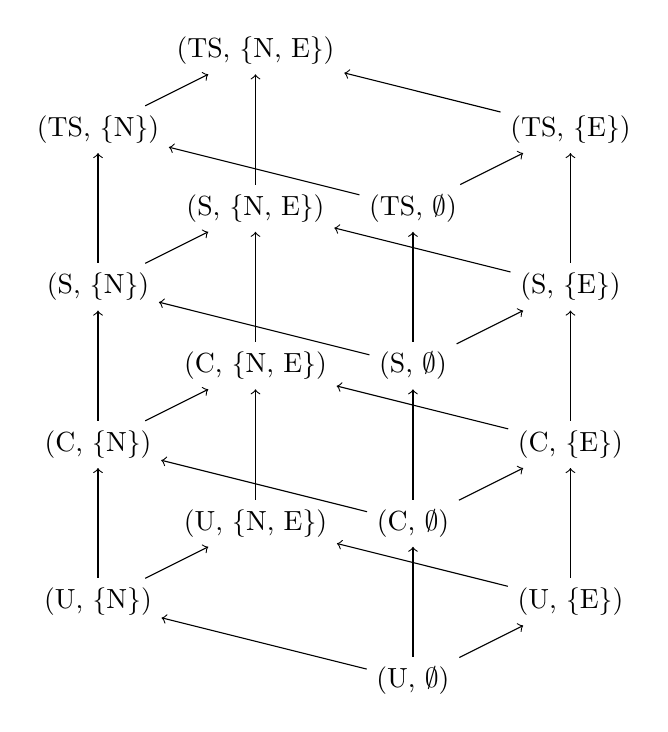
\begin{tikzpicture}
    \node (TSNE) at (2,8) {(TS, \{N, E\})};
    \node (TSE)  at (6,7) {(TS, \{E\})};
    \node (TSN)  at (0,7) {(TS, \{N\})};

    \node (SNE) at (2,6) {(S, \{N, E\})};
    \node (SE)  at (6,5) {(S, \{E\})};
    \node (TS)  at (4,6) {(TS, $\emptyset$)};
    \node (SN)  at (0,5) {(S, \{N\})};

    \node (CNE) at (2,4) {(C, \{N, E\})};
    \node (CE)  at (6,3) {(C, \{E\})};
    \node (S)   at (4,4) {(S, $\emptyset$)};
    \node (CN)  at (0,3) {(C, \{N\})};

    \node (UNE) at (2,2) {(U, \{N, E\})};
    \node (UE)  at (6,1) {(U, \{E\})};
    \node (C)   at (4,2) {(C, $\emptyset$)};
    \node (UN)  at (0,1) {(U, \{N\})};
    \node (E)   at (4,0) {(U, $\emptyset$)};
    \draw[<-] (TSNE) -- (SNE);
    \draw[<-] (TSNE) -- (TSN);
    \draw[<-] (TSNE) -- (TSE);
    \draw[<-] (TSE) -- (SE);
    \draw[<-] (TSN) -- (SN);
    \draw[<-] (TSN) -- (TS);
    \draw[<-] (TSE) -- (TS);

    \draw[<-] (SNE) -- (CNE);
    \draw[<-] (SNE) -- (SN);
    \draw[<-] (SNE) -- (SE);
    \draw[<-] (SE) -- (CE);
    \draw[<-] (SN) -- (CN);
    \draw[<-] (TS) -- (S);
    \draw[<-] (SN) -- (S);
    \draw[<-] (SE) -- (S);

    \draw[<-] (CNE) -- (UNE);
    \draw[<-] (CNE) -- (CN);
    \draw[<-] (CNE) -- (CE);
    \draw[<-] (CE) -- (UE);
    \draw[<-] (CN) -- (UN);
    \draw[<-] (S) -- (C);
    \draw[<-] (CN) -- (C);
    \draw[<-] (CE) -- (C);

    \draw[<-] (UNE) -- (UN);
    \draw[<-] (UNE) -- (UE);
    \draw[<-] (UN) -- (E);
    \draw[<-] (UE) -- (E);
    \draw[<-] (C) -- (E);
  \end{tikzpicture}
  \caption{Retículo de niveles de seguridad.\label{fig:lattice} }
\end{figure}
  \item Sí, $L(\text{Presidente})$ domina a $L(\text{Costo del p.\ nuclear})$ y
    $L(\text{Costo del ejercito})$, por lo que en base a la propiedad-ss, esta
    permitido.
\item No, el mayor no tiene acceso al número de unidades nucleares por que su
  nivel de seguridad no incluye la categoría N. En otras palabras, porque 
  $(\text{C, \{E\}})~\neg\mathsf{dom}~(\text{C, \{N\}})$.
\item Sí, el nivel de seguridad del coronel domina al nivel de ambos objetos.
\item Sí.
\item Ambos pueden, ya que $L(\text{Código Nuclear}) = (\text{TS, \{N\}})$
  domina tanto a (C, \{N\}) (nivel del coronel) como a (U, \{N\}) (nivel del
  soldado), por lo que no contradicen la propiedad-*.
\item Bell-La Padula no garantiza integridad, solo confidencialidad. Esto
  significa que un sujeto con clasificación \textit{Unclassified}, puede borrar
  (accidentalmente o no) información secreta. Para prevenir esto, a veces se
  usa una propiedad-* modificada que requiere $L(s) = L(o)$; es decir, todo
  sujeto puede escribir en su mismo nivel, pero no en mayores.
\end{enumerate}
\end{soln}
\end{document}


